\section{分布式内存对象存储架构和性能分析}

\subsection*{目录}
\frame {
	\frametitle{目录}
    \tableofcontents[currentsection]
}

\subsection*{架构分析}
\begin{frame}
	\frametitle{Plasma集群架构}

	\vspace{-1.5em}
	\begin{columns}[t]
		\column{0.4\textwidth}
		\begin{block}{节点内}
			\begin{itemize}
				\item 基于mmap的共享内存
				\item 无网络开销
				\item 常数延迟读取
			\end{itemize}
		\end{block}
		\begin{block}{节点间}
			\begin{itemize}
				\item 对象分布信息:Redis
				\item Manager拉取对象
				\item \textbf{套接字通信}
			\end{itemize}
		\end{block}
		\column{0.6\textwidth}
		\begin{figure}
			\centering
			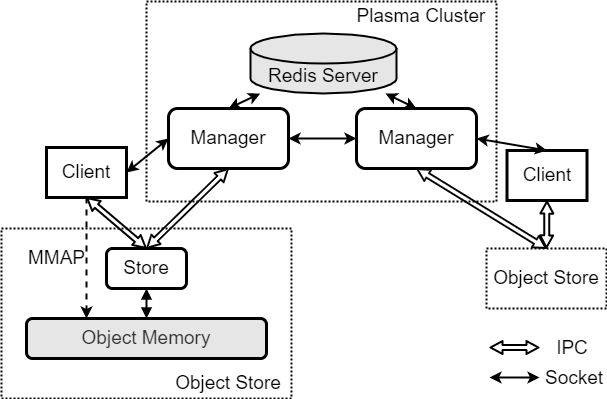
\includegraphics[width=\textwidth]{image/chap02/plasma_arch.png}
			\caption{Plasma集群架构}
		\end{figure}
	\end{columns}

\end{frame}

\subsection*{性能测试和分析}
\begin{frame}
	\frametitle{传输性能测试}

	\begin{columns}[t]
		\column{0.3\textwidth}
		\begin{block}{Plasma vs. Redis}
			\begin{itemize}
				\item 小对象延迟相似
				\item 大对象吞吐低
			\end{itemize}
		\end{block}
		\begin{block}{分析}
			\begin{itemize}
				\item \textbf{套接字通信}
				\item 元数据访问
				\item 本地内存分配
			\end{itemize}
		\end{block}
		\column{0.7\textwidth}
		\begin{figure}
			\centering
			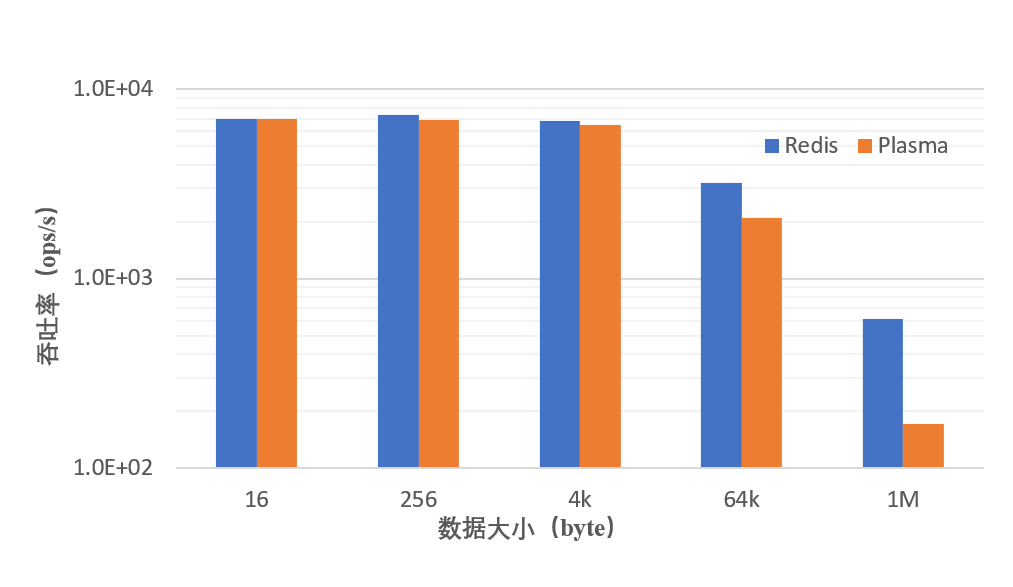
\includegraphics[width=\textwidth]{image/chap02/fetch.png}
			\caption{传输性能测试}
		\end{figure}
	\end{columns}
\end{frame}